\chapter{Weekly Reports \\
\small{\textit{-- Chan, Moks, Ponte}}
\index{weekly reports} 
\index{Chapter!Weekly Reports}
\label{Chapter::Weekly Reports}}

\section{Week Report 11 (11/14/2025)}
\label{sec::W11}

\textbf{Work Completed}
\begin{itemize}
  \item Finalized our decision to shift away from developing or evaluating an online/web-deployed interface and instead keep the system entirely local to the user’s machine. We agreed that a locally hosted web interface is acceptable as an optional convenience layer, since it does not require external deployment.
  \item Updated the System Requirements and Constraints chapters to clarify that the project does not include public hosting, authentication, multi-user access, or large-scale usability studies. Any interface will run locally and remain single-user.
  \item Reviewed all existing use cases and user stories to ensure they still apply under a local-only model, making minor adjustments to remove assumptions about remote access or browser-based UX.
  \item Continued improving the core LLM-to-QUBO translation, validation, and reverse-translation pipeline so that it remains modular and stable regardless of the chosen local interface.
  \item Ensured the architecture description and diagrams are consistent with the local-first direction, where the interface is lightweight and the pipeline remains the primary focus of the system.
\end{itemize}

\textbf{Planned Work for Next Week}
\begin{itemize}
  \item Complete all edits to the Requirements, Use Cases, and Design chapters so they clearly distinguish between the current local-only system and any potential future extension involving a cloud-hosted interface.
  \item Update or regenerate architecture figures, if needed, to illustrate the interaction model for a local UI or a locally hosted web interface running on \texttt{localhost}.
  \item Strengthen unit and integration tests around the pipeline components to ensure reliability during the final demo and report submission.
  \item Begin preparing the demonstration workflow (CLI sequence, notebook cells, or small local web interface walkthrough) for the final presentation.
\end{itemize}

\textbf{Action Items}
\begin{itemize}
  \item Enoch: Review Requirements and Use Case chapters to remove outdated references to deployed web functionality and adjust traceability links accordingly.
  \item Benjamin: Update design text and any interface-related diagrams to emphasize the local interaction model and clarify how a local web interface fits into the architecture.
  \item Kyle: Update Weekly Reports and introductory sections to document the pivot clearly and ensure narrative consistency across earlier weeks and the final report.
\end{itemize}

\textbf{Issues/Risks}
\begin{itemize}
  \item Some older text still references browser-based usability expectations, so careful editing is needed to avoid contradictions in the final draft.
  \item The shift away from a fully featured web interface reduces how much we can say about remote usability or interface testing.
  \item With limited time before the deadline, there is a risk of small mismatches between diagrams, requirements, and implementation if updates are not coordinated.
\end{itemize}

\section{Week Report 10 (11/07/2025)}
\label{sec::W10}

\textbf{Work Completed}
\begin{itemize}
    \item Updated the project budget to include API key costs for OpenAI and D-Wave services.
    \item Met with a D-Wave advisor to discuss the Voyager quantum application and integration feasibility.
    \item Reviewed the fidelity scoring process to ensure consistent metrics across experiments.
    \item Made minor improvements to the project documentation and Use Case traceability.
    \item Configured a GitHub Actions autobuild to create versioned ZIP artifacts (e.g., QuantumOptimizationLLM\_v1.0.1.zip) from the report PDF.
    \item Captured a screenshot of the successful autobuild run for documentation.
\end{itemize}

\textbf{Planned Work for Next Week}
\begin{itemize}
    \item Begin preparing the next progress presentation.
    \item Continue working on validation consistency between translation and reverse translation modules.
\end{itemize}

\textbf{Action Items}
\begin{itemize}
    \item Enoch: Finalize budget documentation and begin drafting presentation slides.
    \item Benjamin: Review and refine current code modules.
    \item Kyle: Continue testing QUBO outputs on the D-Wave hybrid solver and record performance metrics.
\end{itemize}

\textbf{Issues/Risks}
\begin{itemize}
    \item API key expenses could increase with additional solver runs.
    \item Integration between local testing and D-Wave’s Voyager environment may require additional configuration time.
\end{itemize}
\textbf{Directory Packages}
\textbf{Autobuild Screenshot}
\begin{figure}[H]
    \centering
    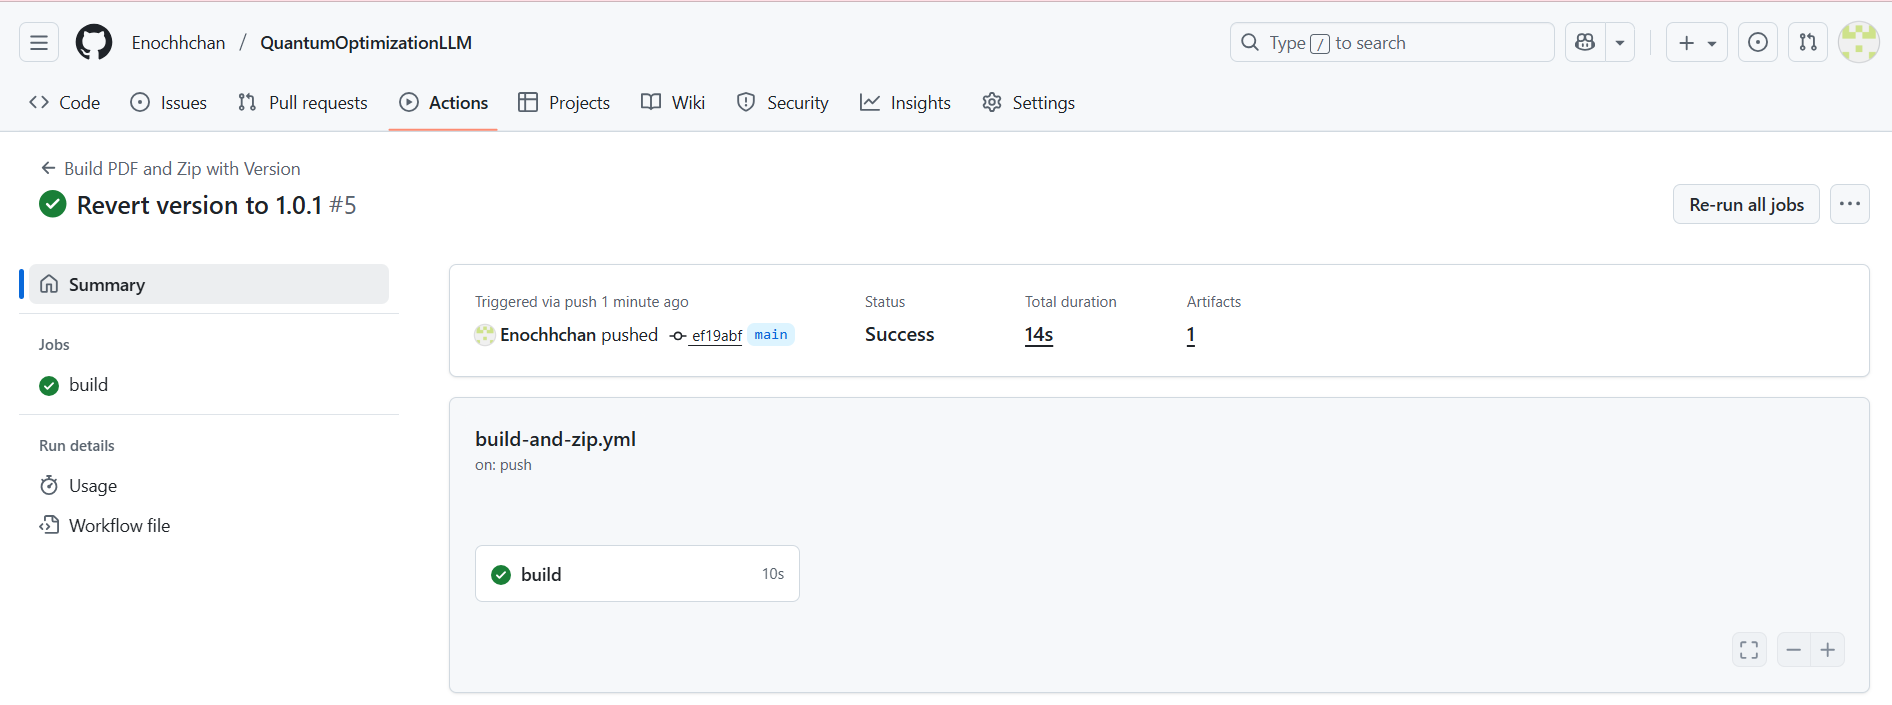
\includegraphics[width=.7\linewidth]{png/build.png}
    \caption{GitHub Actions autobuild producing a versioned artifact \texttt{QuantumOptimizationLLM\_v1.0.1.zip}.}
    \label{fig:AutobuildScreenshot}
\end{figure}


\section{Week Report 9 (10/31/2025)}
\label{sec::W9}

\textbf{Work Completed}
\begin{itemize}
    \item Met with D-Wave technical advisors at 3PM on 10/31/2025.
    \item Created Use Case Diagrams for each use case.
    \item Updated the requirements to include the fact that we are planning to deploy a web interface.
\end{itemize}

\textbf{Planned Work for Next Week}
\begin{itemize}
    \item Introduce a new benchmark problem (Quadratic Assignment) per the request of D-Wave technical advisors.
    \item Experiment with the free capabilities of D-Wave hybrid solvers to validate the structure of our QUBO.
    \item Begin developing the web interface.
    \item Refine Use Case diagrams.
\end{itemize}

\textbf{Action Items}
\begin{itemize}
    \item Enoch: Refine the Use Case diagrams.
    \item Benjamin: Determine how the web interface should be developed.
    \item Kyle: Incorporate the Quadratic Assignment problem into the rest of the experiments and begin testing.
\end{itemize}

\textbf{Issues/Risks}
\begin{itemize}
    \item API costs of running additional experimentation.
\end{itemize}

\section{Week Report 8 (10/24/2025)}
\label{sec::W8}

\textbf{Work Completed}
\begin{itemize}
  \item Finished Activity Diagrams for each of the use cases.
  \item Connected with a D-Wave representative (Jacob van Leenen) in regards to hybrid solver access.
  \item Corrections were made to the document based on feedback.
\end{itemize}

\textbf{Planned Work for Next Week}
\begin{itemize}
  \item Meet with the D-Wave representative.
  \item Begin working on Use Case diagrams.
  \item Continue progress on the midterm presentation.
\end{itemize}

\textbf{Action Items}
\begin{itemize}
  \item Enoch: Create Use Case diagrams.
  \item Benjamin: Organize the meeting with the D-Wave representative.
  \item Kyle: Work on the midterm presentation.
\end{itemize}

\textbf{Issues/Risks}
\begin{itemize}
  \item Modular design may need tweaks.
  \item Midterm timeline pressure; coordination needed to keep UML and implementation in sync.
\end{itemize}

\section{Week Report 7 (10/17/2025)}
\label{sec::W7}

\textbf{Work Completed}
\begin{itemize}
  \item Created Activity Diagrams for essential use cases and validated them against CRC cards.
  \item Refined object-oriented design; aligned class responsibilities with use case flows.
  \item Updated midterm deliverables (figures/tables).
\end{itemize}

\textbf{Planned Work for Next Week}
\begin{itemize}
  \item Finalize Activity Diagrams and trace them to all use cases and requirements.
  \item Set up autobuild and versioning for the Hello World prototype (target: v0.1.\#\{changelist\}).
  \item Continue searching for potential hybrid/quantum solvers.
\end{itemize}

\textbf{Action Items}
\begin{itemize}
  \item Enoch: Finalize OO design; ensure UML and code skeletons align.
  \item Benjamin: Start module implementation; configure autobuild/versioning pipeline.
  \item Kyle: Compile Activity Diagrams into the report; draft Week 7 documentation updates.
\end{itemize}

\textbf{Issues/Risks}
\begin{itemize}
  \item Limited access to hybrid hardware solver.
  \item Midterm timeline pressure; coordination needed to keep UML and implementation in sync.
  \item Ensuring traceability from CRC \textrightarrow{} Activity Diagrams \textrightarrow{} Use Cases \textrightarrow{} Requirements.
\end{itemize}

\section{Week Report 6 (10/9/2025)}
\label{sec::W6}

\textbf{Work Completed}
\begin{itemize}
    \item Created CRC cards that demonstrate our initial OO design for the program.
    \item Formulated Use Cases and began going through them with our CRC cards to ensure the modular design is sufficient.
    \item Ran preliminary QUBO translation tests on D-Wave's exact solver to evaluate QUBO validity.
\end{itemize}

\textbf{Planned Work for Next Week}
\begin{itemize}
    \item Begin working on Activity Diagrams for the essential use cases.
    \item Continue working on midterm deliverables.
    \item Make adjustments to OO design if necessary.
\end{itemize}

\textbf{Action Items}
\begin{itemize}
    \item Enoch: Evaluate the modular design against use cases.
    \item Ben: Prepare midterm deliverables such as figures and tables.
    \item Kyle: Create the Activity Diagrams for essential use cases.
\end{itemize}

\textbf{Issues/Risks}
\begin{itemize}
    \item Unsure of the suffiency of our current OO design.
    \item Still have concerns regarding how we will get access to D-Wave's quantum/hybrid solvers.
\end{itemize}

\section{Week Report 5 (10/3/2025)}

\textbf{Work Completed}
\begin{itemize}
    \item Progressed on object-oriented refactoring by integrating modular translation, validation, and fidelity components to an extent.
    \item Expanded experiment dataset to include diverse prompt variations across all canonical problem types.
    \item Generated draft figures and tables summarizing schema validity, fidelity scores, and solver compatibility for midterm deliverables.
\end{itemize}

\textbf{Planned Work for Next Week}
\begin{itemize}
    \item Incorporate reverse translation and semantic fidelity scoring into the experiment pipeline.
    \item Run preliminary QUBO translation tests on simulators to evaluate solver readiness.
    \item Polish midterm deliverables with finalized figures, tables, and updated methodology/results chapters.
\end{itemize}

\textbf{Action Items}
\begin{itemize}
    \item Enoch: Implement reverse translation functions and fidelity scoring integration.
    \item Benjamin: Conduct initial QUBO translation and solver tests; refine experiment logging for semantic metrics.
    \item Kyle: Compile updated figures/tables into the report and draft midterm results discussion.
\end{itemize}

\textbf{Issues/Risks}
\begin{itemize}
    \item Risk of incomplete semantic fidelity scoring before midterm deadline.
    \item Solver access and runtime limits may restrict depth of QUBO evaluation.
    \item Continued concern about API costs and token usage during extended testing.
\end{itemize}

\section{Week Report 4 (09/25/2025)}

\subsubsection{Work Completed}

\begin{itemize}
  \item Implemented Team Assignment experiments and added prompt templates/validators. 
  \item Began restructuring codebase with object-oriented design (class diagrams, UML sketches). 
  \item Working to integrate preliminary object classes into experiment runner.  
\end{itemize}

\subsubsection{Planned Work for Next Week}

\begin{itemize}
  \item Finalize object-oriented refactor with fully modular translation and validation components. 
  \item Expand testing dataset to larger prompt variations across all five canonical problem types. 
  \item Prepare draft figures and tables for midterm deliverables. 
\end{itemize}

\subsubsection{Action Items}

\begin{itemize}
  \item Enoch: Complete UML diagrams and begin coding core classes. 
  \item Benjamin: Refactor experiment runner to integrate modular classes and ensure compatibility. 
  \item Kyle: Consolidate Team Assignment results, update report sections, and draft figures for midterm check-in. 
\end{itemize}

\subsubsection{Issues/Risks}

\begin{itemize}
  \item OOP refactor introduces risk of breaking existing scripts — testing and documentation required. 
  \item API usage and token costs continue to be a concern for extended experiments. 
\end{itemize}

\section{Week Report 3 (09/19/2025)}

\subsubsection{Work Completed}
\begin{itemize}
  \item Conducted initial TSP and Graph Coloring experiments. 
  \item Logged lower success rates and higher variability compared to Knapsack. 
  \item Began drafting Results section outline. 
\end{itemize}

\subsubsection{Planned Work for Next Week}
\begin{itemize}
  \item Implement Team Assignment experiments. 
  \item Restructure codebase with object-oriented design. 
\end{itemize}

\subsubsection{Action Items}
\begin{itemize}
  \item Enoch: Begin UML design for modular refactor. 
  \item Benjamin: Continue expanding dataset and logs. 
  \item Kyle: Extend experiments to Team Assignment. 
\end{itemize}

\subsubsection{Issues/Risks}
\begin{itemize}
  \item Lower success rates in Graph Coloring/TSP highlight model limitations. 
  \item Risk of inconsistency across repeated runs. 
\end{itemize}

\section{Week Report 2 (09/12/2025)}

\subsubsection{Work Completed}
\begin{itemize}
  \item Reproduced Knapsack and Seating Assignment experiments from prior group’s work. 
  \item Hardened schema validator to detect missing objectives and malformed constraints. 
  \item Implemented logging to CSV for prompt ID, status, latency, and fidelity score. 
  \item Drafted methodology extension and pinned dependencies. 
\end{itemize}

\subsubsection{Planned Work for Next Week}
\begin{itemize}
  \item Extend experiments to TSP and Graph Coloring. 
  \item Add timing metrics for translation, validation, and fidelity stages. 
  \item Define clear success criteria for experiments. 
  \item Generate figures for success rates, fidelity, and latency. 
\end{itemize}

\subsubsection{Action Items}
\begin{itemize}
  \item Enoch: Create TSP and Graph Coloring templates and validators. 
  \item Benjamin: Add timers and generate plots. 
  \item Kyle: Integrate results and update the report. 
\end{itemize}

\subsubsection{Issues/Risks}
\begin{itemize}
  \item API rate limits and costs may restrict experiments. 
  \item Model variability affects schema validity. 
  \item Dependency drift can cause errors. 
\end{itemize}

\section{Week Report 1 (09/05/2025)}

\subsubsection{Work Completed}
\begin{itemize}
  \item Reviewed the IEEE paper of the previous group, \cite{sato2025trustworthy} and studied the LLM-to-QUBO translation pipeline. 
  \item Examined schema validation, reverse translation, and fidelity scoring as described in the paper. 
  \item Drafted the Introduction chapter with team member bios. 
  \item Created the Weekly Reports appendix and updated the document history. 
\end{itemize}

\subsubsection{Planned Work for Next Week}
\begin{itemize}
  \item Reproduce a subset of experiments from the IEEE paper, starting with Knapsack and Seating Assignment. 
  \item Configure the Python environment and experiment scripts. 
  \item Begin drafting an extended methodology section. 
\end{itemize}

\subsubsection{Action Items}
\begin{itemize}
  \item Enoch: Set up Python environment and dependencies. 
  \item Benjamin: Re-implement experiment logging scripts. 
  \item Kyle: Draft updated methodology text and maintain version control. 
\end{itemize}

\subsubsection{Issues/Risks}
\begin{itemize}
  \item Difficulty replicating results without full access to prior environment. 
  \item Latency and API limits could slow experimentation. 
\end{itemize}


